\section{Résumé des 8 premières semaines}
Le but ici va être de résumé ce qui a été dit, donc avec les méthodes théorème (ceux très importants donc il en manque (voir les pdf résumé sur moodle)). 
\subsection{Equation différentielle}
\begin{parag}{Equation à variable séparée}
    Lorsqu'on à une équation du type $f\left(x\right)\cdot y' = g\left(x\right)$ on a comme solution:
   \begin{equation*} f\left(y\right)\cdot \frac{dy}{dx} = g\left(x\right) \implies \int f\left(y\right)dy = \int g\left(x\right)dx \end{equation*} 
   Il suffit ensuite de résoudre les deux primitives et ensuite de simplifier pour $y$.
\end{parag}
 
\begin{parag}{Equation différentielle linéaire du premier ordre}
    Si on a une équation du type:
    \begin{equation*} y'\left(x\right) + p\left(x\right)y\left(x\right) = f\left(x\right)  \end{equation*}
    Il y a plusieurs cas:
    \begin{subparag}{Cas des constantes}
        si $p\left(x\right)$ et $f\left(x\right)$ sont des constantes,Alors on pose pour $p\left(x\right)$
        \begin{equation*} \frac{y'\left(x\right)}{y\left(x\right)} -p\left(x\right) \end{equation*}
        Et donc on résoud $\int \frac{dy}{y} = -\in^{\left(x\right)}$ ce qui nous donne comme solution générale:
        \begin{equation*} y\left(x\right) = Ce^{-P\left(x\right)} \end{equation*}
    \end{subparag}
    
\end{parag}
\begin{parag}{Méthode de la variation de la constante}
    On va ici lister les étapes comme ci c'était un algorithme:
    \begin{subparag}{Résoudre l'équation homogène associée}
        \begin{equation*} y_h'\left(x\right) + p\left(x\right)y_h\left(x\right) = 0 \end{equation*}
        On peut résoudre par en séparant les variables ce qui donne:
        \begin{equation*} y_h\left(x\right) = Ce^{-\int^{\left(x\right)} \end{equation*}
    \end{subparag}
    \begin{subparag}{Faire varier la constante}
        On remplace la constante $C$ par une fonction $c\left(x\right)$
        \begin{equation*} y_p\left(x\right) = c\left(x\right) \cdot e^{-\int p\left(x\right)dx} \end{equation*}
       
    \end{subparag}
    \begin{subparag}{Remplacer $y_p$ dans l'équation initiale}
        On calcule la dérivée:
        \begin{equation*} y_p'\left(x\right) = c'\left(x\right) \cdot  e^{-\int p\left(x\right)dx} + c\left(x\right)\cdot \left(-p\left(x\right)e^{-\int p\left(x\right) dx}\right) \end{equation*}
       En simplifiant on obtient:
       \begin{equation*} c'\left(x\right) \cdot e^{-\int p\left(x\right) dx} = f\left(x\right)\end{equation*}
    \end{subparag}
    \begin{subparag}{Résoudre pour $c\left(x\right)$}
        \begin{equation*} c'\left(x\right) = f\left(x\right) \cdot  e^{p\left(x\right)dx} \end{equation*}
        \begin{equation*} c\left(x\right) = \int f\left(x\right) \cdot  e^{\int p\left(x\right) dx} \end{equation*}
    \end{subparag}
    \begin{subparag}{Donner la solution particulière}
        \begin{equation*} y_p\left(x\right) = c\left(x\right) \cdot  e^{-\int p\left(x\right) dx} \end{equation*}
        
    \end{subparag}
    Donc on a comme solution générale:
    \begin{equation*} y\left(x\right) = y_h\left(x\right) + y_p\left(x\right) \end{equation*}
    Ou alors si on veut juste speedrun:
    \begin{equation*} y\left(x\right) = C\cdot e^{-\int p\left(x\right) dx} + \left(\int f\left(x\right) \cdot  e^{\int p\left(x\right) dx}dx\right) \cdot  e^{-\int p\left(x\right) dx} \end{equation*}
    
\end{parag}
\begin{parag}{Equation différentielle du second ordre}
    Donc ici c'est pour toute les équations du type:
   \begin{equation*} y''\left(x\right) + p\left(x\right)y'\left(x\right) + q\left(x\right)y\left(x\right) = 0 \end{equation*} 
  Lorsque les fonctions $p$ et $q$ sont juste des coefficients constants, on a ce qu'on appelle une EDL2 à coefficient constants. Pour résoudre ce type d'équation il suffit de résoudre l'équation caractéristique qui est donnée par:
  \begin{equation*} \lambda^2 + p\lambda + q = 0 \end{equation*}
  Lorsque tu trouves les solutions pour $\lambda$ on a:
  \begin{equation*} y\left(x\right) = \begin{cases} C_1e^{ax} + C_2 e^{bx} \; \; \text{ si } a \neq b, \; \; a, b \in \mathbb{R} \\
      C_1e^{ax} + C_2xe^{ax} \; \; \text{ si } a = b\\
  C_e^{\alpha x}\cos \beta x + C_2e^{\alpha x} \sin \beta x \; \; \text{ si } a = \alpha + i \beta = \overline{b} \notin \mathbb{R} \end{cases}
  \end{equation*}
\end{parag}
\begin{parag}{Méthode de résolution de EDL2}
    Pour résoudre on trouve en premier lieu deux solutions linéairement indépendantes de l'équation homogène
    \begin{equation*}  y''\left(x\right) + p\left(x\right)y'\left(x\right) + q\left(x\right)y = 0 \end{equation*}
    Après avoir trouvé les deux solutions $y_1$ et $y_2$, on va utiliser le Wronskien avec la méthode de la variation de la constante.
    On a que 
    \begin{equation*} y_p\left(x\right) = u_1\left(x\right)y_1\left(x\right) + u_2\left(x\right)y_2\left(x\right) \end{equation*}
    avec pour nos deux $u\left(x\right)$:
   \begin{align*} u_1\left(x\right) = - \int\frac{y_2\left(x\right)f\left(x\right)}{W\left(x\right)}\\
   u_2\left(x\right) = \int \frac{y_1\left(x\right)f\left(x\right)}{W\left(x\right)}\end{align*} 
   On a donc pour solution particulière:
   \begin{equation*} y_p\left(x\right) = u_1\left(x\right)y_1\left(x\right) + u_2\left(x\right)y_2\left(x\right) \end{equation*}
   Et pour la solution générale:
   \begin{equation*} y\left(x\right) = C_1y_1\left(x\right) + C_2y_2\left(x\right) + y_p\left(x\right) \end{equation*}
    je colle ici la slide de la prof sur la marche à suivre:
    \begin{figure}[h!]
       \centering 
    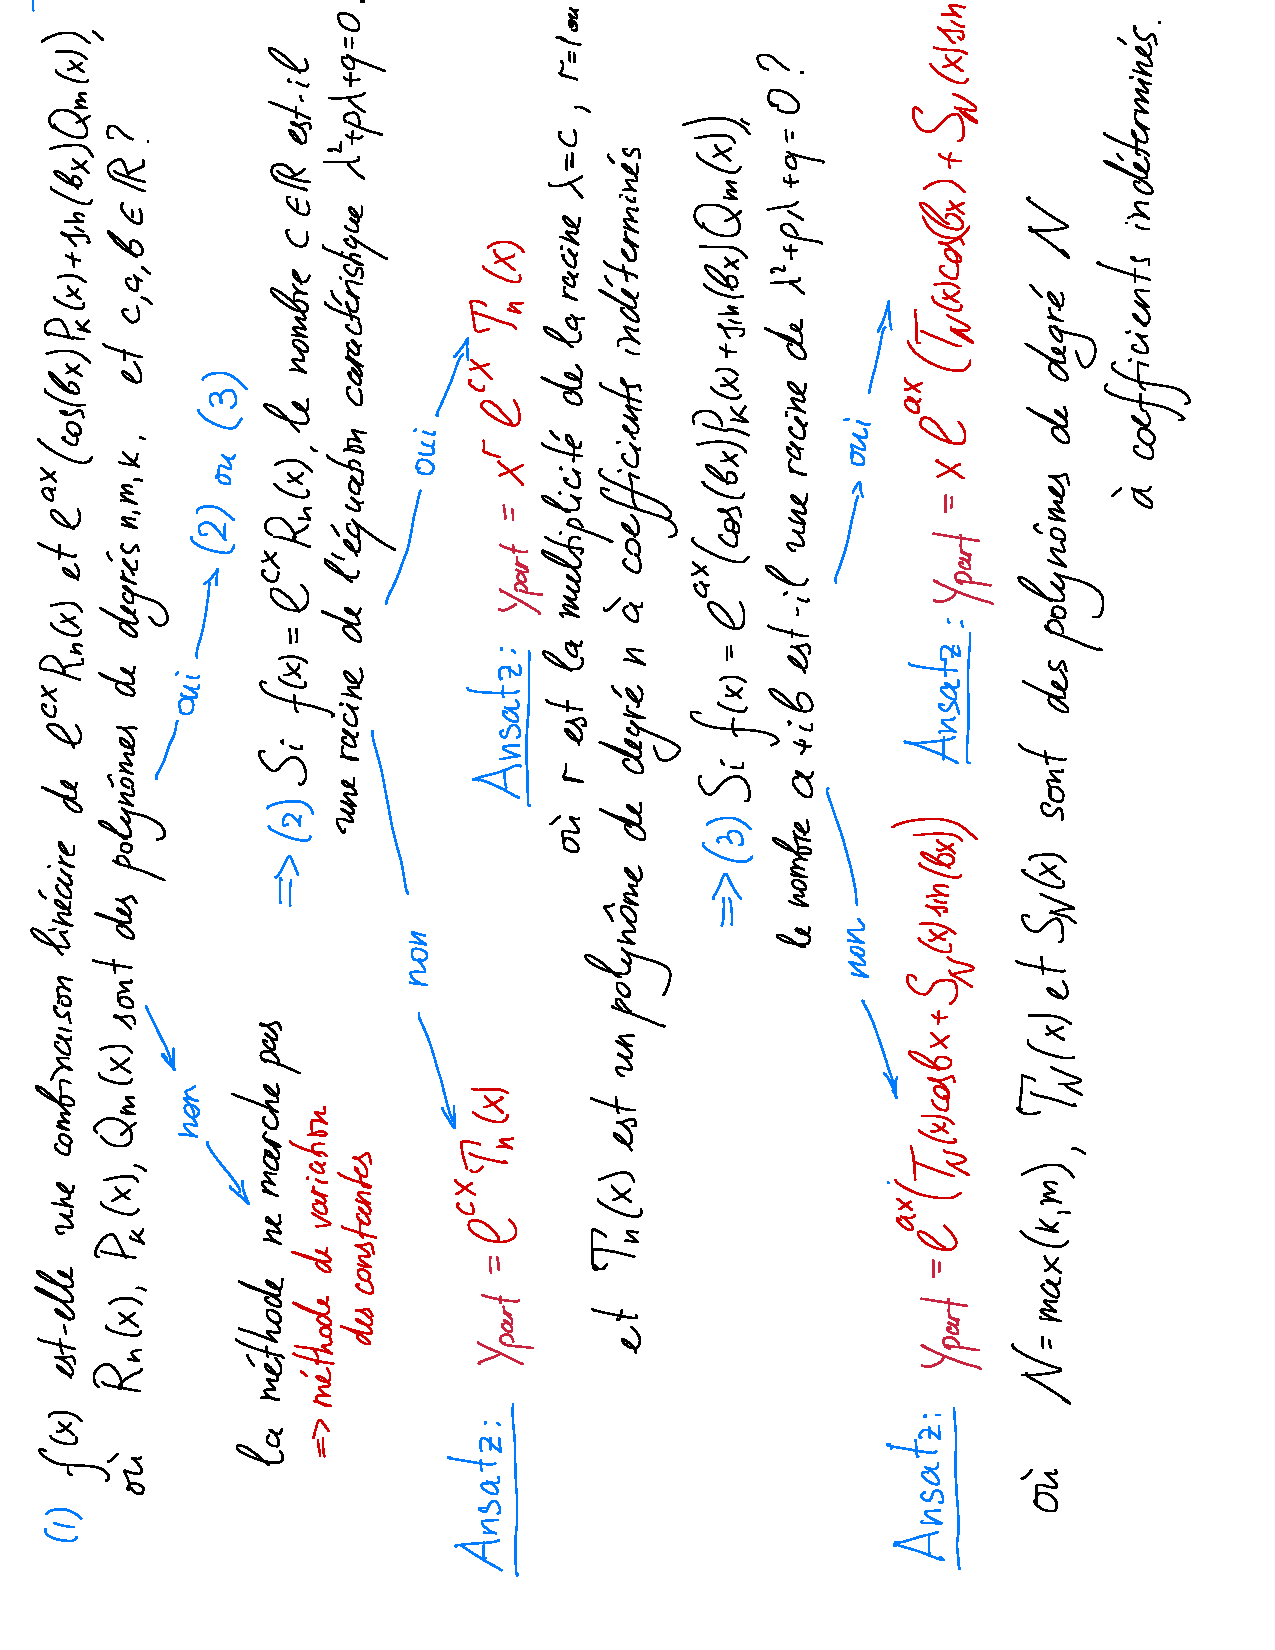
\includegraphics[angle=270, scale=0.6]{resuméEDL2.pdf}
    \end{figure}
    
    
\end{parag}









